\documentclass[a4paper,10pt]{article}

\usepackage{amsmath,graphicx,fullpage,microtype,hyperref,subfig,hypcap}

\DisableLigatures{encoding=*,family=*}
\numberwithin{equation}{section}
\setlength{\parindent}{0px}
\widowpenalty=300
\clubpenalty=300
\hyphenpenalty=300
\hypersetup{colorlinks,citecolor=black,filecolor=black,linkcolor=black,urlcolor=black}

\begin{document}

\label{sec:Cover Page}
\addcontentsline{toc}{section}{Cover Page}

Laurens Bogaardt \hfill \href{http://www.lu.se}{Lunds Universitet}\\
\href{mailto:gec11lbo@student.lu.se}{gec11lbo@student.lu.se} \hfill Master's Thesis\\
 \hfill 29-05-2012\\

\vspace{3cm}

\begin{center}
\begin{LARGE}
\begin{bf}
The Evolutionary Foundation of Probability Weighting and Hyperbolic Discounting
\end{bf}
\end{LARGE}
\end{center}

\vspace{0cm}

\begin{center}
\begin{large}
\begin{bf}
And Their Intimate Connection
\end{bf}
\end{large}
\end{center}

\vfill

\begin{center}
\begin{minipage}[t]{0.7\textwidth}
\begin{bf}
Abstract
\end{bf}
\newline
\newline
In this paper, we delve into the evolutionary foundation of both probability weighting and hyperbolic discounting. We argue that it is evolution which selects between various kinds of people those who have the optimal preference profile. As such, utility functions and behavioural biases can be explained from an evolutionary perspective. We also argue that there may be an intimate connection between hyperbolic discounting and probability weighting. This follows from the similarities between these two deviations from what normative economic theory would consider 'rational'. Following the suggestion of this intimate connection, we analyse a model which is capable of explaining why probability weighting may have been advantageous for our ancestors and we look whether we can reinterpret this model to also include hyperbolic discounting. This turns out to be difficult, however, as an analysis of the properties of our model makes clear. 
\end{minipage}
\end{center}

\vspace{.4cm}

\begin{center}
\begin{minipage}[t]{0.7\textwidth}
\begin{bf}
Acknowledgements
\end{bf}
\newline
\newline
The author wishes to thank Jerker Holm for the supervision during the writing of this paper and for helping make difficult parts more understandable. The author also wishes to thank Niels Kouwenhoven and Matt van der Gronde for the discussions which helped materialise the concepts within this paper.
\end{minipage}
\end{center}

\vspace{.6cm}

\newpage

\phantomsection
\label{sec:Contents}
\addcontentsline{toc}{section}{Contents}
\renewcommand{\contentsname}{Contents\\} 
\tableofcontents

\newpage

\section{Introduction}
\label{sec:Introduction}
\subsection{Behavioural Economics}
\label{sec:Behavioural Economics}

Behavioural economics has in recent times caused a shift in the focus of economists from theoretically rational models to empirically correct models. The purpose of behavioural economics is not to create a normative theory of human behaviour, but rather to produce a descriptive theory adequate to deal with certain counter-intuitive behaviour seen in many situations \cite{Kahneman1990}. For example, it seems people are willing to drive across town to save $5$ euro on a $15$ euro calculator, but not to save $5$ euro on a $125$ euro jacket \cite{Kahneman1984}. Research is now being done on how this irrational economic behaviour can be explained by psychological tendencies. The clear divide between psychology and economics has subsequently become more blurry and many suggestions from psychology for more realistic human behaviour have entered into the field of economics. Mental accounting describes how people categorise financial activities in their brain in a similar manner to how accountants in firms categorise such activities and can explain, for example, why cab drivers stop work early on a good day while continue working longer on rainy days \cite{Wilkinson2008}. The problem which normative economic theory has with this behaviour is that it would be wiser to work as long as possible on a good day in which there is a lot of money to be made. To maximise pay-offs, it is rational to work relatively more on such good days than on bad days. The availability heuristic says that people determine the likelihood of an event occurring by the ease at which it comes to mind and the representativeness heuristic describes how people judge the probability of an object A belonging to a class B by seeing how much A resembles B \cite{Tversky1974}. These tendencies can help explain why we see certain irrational behaviour; behaviour which does not directly lead to utility maximisation. However, it does not explain why humans show this type of behaviour in the first place. We have merely pushed the question of explaining the data one step further, from the field of economics to the field of psychology. We have found a proximate cause for such seemingly irrational behaviour in these psychological tendencies, but we still lack an ultimate cause. It is the purpose of evolutionary psychology and evolutionary game theory to provide such an ultimate cause. The idea is that behaviour which is advantageous to the survival of the individual will spread in the population and become dominant. A more precise definition of this view will be given later in the description of our model. One needs only to show how certain behaviour, which normative economics may consider irrational, can be advantageous to human ancestors, in order to explain why this behaviour persists today. Evidence that this view of behaviour being shaped in our evolutionary past is correct follows from experiments with animals. When examining loss-aversion in capuchin monkeys, Chen et al. found that the behaviour was strikingly similar to that of humans. They conclude that, because capuchin monkeys lack the ability of social learning, this behaviour must have had a early-evolutionary origin and be innate to human ancestors \cite{Chen2006}. Furthermore, studies on rats have shown that they exhibit the same irrational, hyperbolic way of discounting the future as we humans do, but more on this particular topic later \cite{Richards1997}.\\
\\
Coming back to the examples mentioned earlier, we can posit that mental accounting simplifies decision making by creating clear divisions between activities. Furthermore, representativeness leads to accurate predictions in most common situations; situations in which the resemblance between object A and class B really does say something about their connection. In general, we can say that applying heuristics greatly reduces complex tasks; something evolution would favour. Only in very specific situations do these heuristics lead to strong biases, as illustrated by the example of the cab driver \cite{Tversky1974}. Furthermore, it has been shown that a form of loss-aversion may be beneficial in situations with strategic interaction. Loss-aversion leads to a certain toughness in bargaining, which may cause the opponent in a Nash-bargaining game to adjust his behaviour in a way that would benefit the biased bargainer \cite{Huck2005, Heifetz2004}. If we view this Nash-bargaining game as representative of situations in which human ancestors found themselves, we conclude that loss-aversion would survive the evolutionary process in the long-run.\\
\\
Having given some examples of irrational economic behaviour and their underlying psychological tendencies, we have presented a number global reasons for why this irrational behaviour may be advantageous when viewed through the lens of natural selection. We will now turn to another theory which describes how humans make decisions: Prospect Theory. In particular, we will discuss probability weighting. It is one of the main purposes of the rest this paper to provide an account of why this behaviour, as well, may be advantageous in an evolutionary setting.


\subsection{Probability Weighting}
\label{sec:Probability Weighting}

When examining data on gambles, it seems people do not adhere to the normative theory of expected utility. As such, they do not maximise their utility. Moreover, people seem to violate the independence axiom and are reluctant to back away from a loosing bet, as illustrated by their reluctance to sell a falling stock \cite{Wilkinson2008}. In 1979, Kahneman and Tversky published their seminal paper on Prospect Theory, in which they developed a theory of human behaviour under risk and uncertainty which was capable of explaining the empirical data \cite{Kahneman1979}. The authors proposed two main alterations to the expected utility theory: the value function would replace the standard utility function and weighted probabilities would be used in gambles, or what they called prospects.\\
\\
The key feature of the value function is its reference point. People do not look at their total wealth and total utility when making a financial decision, but frame every separate action using their present state as a null-point or reference point. From there, a loss will decrease utility temporarily while a gain will increase utility temporarily, until a new reference-point is established. Another part of Prospect Theory is the diminishing sensitivity for both gains and losses. Finally, the value function also includes loss aversion, by making the part in the negative somewhat steeper than the part in the positive.\\
\\
From an evolutionary perspective, these three features all make sense. We had already discussed loss-aversion above, which can be advantageous in situations with strategic interaction. The fact that people view gains and losses as compared to a reference point also makes sense when one realises that evolution is an ever increasing arms race in which you are running to stand still. It does not matter how good you are, only that you are better than the rest. The research by Chen et al. on capuchin monkeys also revealed this reference dependence \cite{Chen2006}. Finally, the diminishing sensitivity can be explained by examining the environment in which animals struggle for life. In a paper by McDermott et al., the authors build a model where animals need a certain number of resources to survive to the next period \cite{McDermott2008}. In a situation with some uncertainty, animals who are at the verge of dying may need to take high risks in order to have at least a small chance of surviving. For these animals, it's all or nothing. As such, the marginal effect of losses on survival diminishes as the potential losses get larger.\\
\\
The second, and for the present discussion the most important part of Prospect Theory is the probability weights which people seem to use when judging gambles. Although the theory has been adjusted and updated in more recent papers, the general idea is that people overweight prospects with low probability and underweight prospects with almost certain probability. An example of the first case is the betting on long-shot horses in horse racing; even though there is only a small chance that these horses will win, people behave as if the probability is higher. In their 1992 paper, Kahneman and Tversky propose a weighting function which has the following form \cite{Tversky1992}:

\begin{equation}
\label{eq:myWeight}
\pi(p, \gamma)=\frac{p^{\gamma}}{(p^{\gamma}+(1-p)^{\gamma})^{\frac{1}{\gamma}}}
\end{equation}\\

The factor $\gamma$ in this equation determines the level of weighting applied; for $\gamma=1$, the function is linear and the subjective probability $\pi$ is equal to the true probability $p$. For values lower than $\gamma=1$, over- and underweighting is observed in accordance with Figure~\ref{fig:Graph1.pdf} on the following page.\\
\\
Probability weighting has not only been observed in humans, but also in other animals. Similar to the discovery of loss-aversion in monkeys, this provides evidence to back up our initial claim that evolution is responsible for the psychological tendencies we have and ultimately for the irrational economic behaviour we observe. But is probability weighting also advantageous? Would it survive in an evolutionary setting? One of the three key points this paper wants to propose is an extension of a previous model in which probability weighting is evolutionarily advantageous. Before we move on to this model, we continue with our introduction into behavioural economics and discuss hyperbolic discounting.

\begin{figure}[h]
\begin{center}
\leavevmode
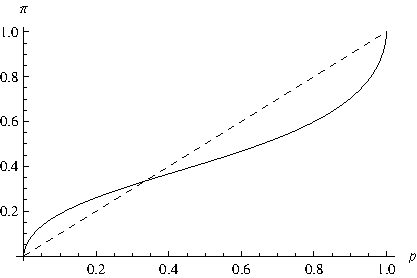
\includegraphics[scale=1.2]{Graph1.pdf}
\caption{Prospect Theory probability weighting for $\gamma=0.6$.}
\label{fig:Graph1.pdf}
\end{center}
\end{figure}


\subsection{Hyperbolic Discounting}
\label{sec:Hyperbolic Discounting}

When rewards are realised at a time later than the present, the benefit of such rewards are discounted. In the market place, this is often done using the interest rate such that the present value of the reward is determined by calculating what reward in the present, together with its compound interest over time, would equal the future reward in terms of benefit. In a more social setting, a similar behaviour is reasonable when there is an uncertainty involved with the realisation of the reward. If rewards further in the future are less certain, their present value should be less high. For a constant uncertainty rate through time, or a constant interest rate, the shape of the discount function, which describes by how much to discount a future reward, should be exponentially decaying.

\begin{equation}
\label{eq:myExponential}
f(t) = f_0 \times \delta^{t} \hspace{.4cm} \text{where} \hspace{.2cm} 0<\delta<1
\end{equation}\\

Several experiments, however, have shown that the shape of this function according to actual human behaviour is more closely related to a hyperbolic function \cite{Green1994, Rachlin1991}. In this case, the subjective value from the present to the near future makes a large drop, i.e. people discount the near future heavily. For example, when you are given the option between $1$ euro now or $1$ euro tomorrow, you have a very strong preference for the $1$ euro now. Simultaneously, the difference in value associated with two rewards in the far future, separated by the same amount of time, is only small\footnote{In mathematics, the term 'hyperbolic' refers to the particular functional form $u(t, k)=\frac{u_0}{1+k t}$. Initial experiments used this functional form to fit their data \cite{Richards1997}. However, in recent times, economists use the term hyperbolic to merely mean the behaviour just described: large drops from the present to the near future and smaller drops in the far future.}. This means people do not care all that much about either obtaining $1$ euro in one year time or obtaining $1$ euro in one year plus one day. Put more simply, the discount factor is not constant, such as the interest rate or the uncertainty rate is constant, but increases for periods further into the future.\\
\\
One of the important implications of hyperbolic discount function is that two functions at different time periods may cross. This means that there is a possibility of preference reversal in which a person would first favour A over B, but as some time passes, changes his mind and favours B over A\footnote{One may wonder whether such a reversal of preferences is not so detrimental to optimal decision making that it could never survive in evolution through natural selection. As a reply to this, Netzer posits that animals where never able to change their minds in the type of situations in our evolutionary past we are considering \cite{Netzer2009}. Dynamic inconsistencies could never arise back then because decisions were irreversible, while in recent times, through the market place, decision have increasingly become more reversible. As such, in the modern world, hyperbolic discounting truly does lead to dynamic inconsistencies and the changing of one's mind.}. Similar to the discovery of loss-aversion among capuchin monkeys, Richards et al. found hyperbolic discounting to also be present in rats, suggesting a similar evolutionary mechanism for this behaviour \cite{Richards1997}.\\
\\
Let us examine one possible mechanism for the occurrence of hyperbolic discounting suggested by Sozou\footnote{A similar account is provided by Robsons, who looks at the aggregate uncertainty concerning survival rates to explain the hyperbolic shape of the discount function \cite{Robson2009}.}. For simplicity, let us assume there is no uncertainty regarding the realisation of a reward in the future if one is still alive. The only factor, in that case, that would cause future rewards to be less beneficial to the biological fitness of an animal is the chance that such an animal has died by the time the reward could potentially be realised. The theory in evolutionary biology which deals with such situations is called Life History Theory. In this framework, it is analysed how an animal can best spread out resources and mating opportunities over its lifetime. Following the uncertainty about being alive at some moment in the future, created by environmental hazards, it is often better to have a bias towards the present. If the hazard rate is a known constant, discounting future rewards should be done in a exponential manner as in Equation~\ref{eq:myExponential}. However, throughout evolutionary times, the hazard rate was not always the same and a newborn would not know into what kind of environment he was born. In that case, there is some uncertainty about the hazard rate and the optimal shape of the discount function may no longer be exponential. This approach suggests one possible explanation for hyperbolic discounting\footnote{There are other ideas about the origin of the hyperbolic discount function as well. Notably, Lehmann and Rousset determine the best way to discount future rewards when genetic drift is included, i.e. when the geographical spread of animals and their kin becomes important. They find that the function departs from the standard exponential function, possibly towards a more hyperbolic shape \cite{Lehmann2011}.}. According to Sozou, the hazard rate is initially not known by newborn animals. With time, more information about the specific hazard rate is discovered as the animals learn in what kind of environment they actually live. With this additional information, they update their idea about the hazard rate and change the shape of the discount function for the remaining time. Following some basic assumptions, Sozou shows that, in this case, a hyperbolic discount function is optimal \cite{Sozou1998}.\\
\\
As was rightfully observed by Dasgupta, however, this does not account for the type of preference reversal seen in most empirical data \cite{Dasgupta2005}. If people apply a hyperbolic discount function to future rewards, they may at one moment prefer A over B, while at a later time reverse their preference and go for B instead. This type of dynamic inconsistency arises because two hyperbolic discount functions can cross at different points in time. To see why this cannot occur under the function proposed by Sozou, consider what happens to the discount function, which started out hyperbolic, when some time has passed. The 'present' moves along the curve to the right and the discount function itself rescales to unity, conditional on still being alive at that moment. That is because a resource which was initially expected at some moment in the future, and therefore discounted, is now in the present, and therefore should no longer be discounted. The part of the discount function which lies in the future is no longer the full hyperbolic function, but merely its flat tail. This follows from the fact that the discount rate is age-dependent according to Sozou, who suggested that the hyperbolic shape relies on an updating of the discount rate with age, as more information becomes available to the animal. As the discount function at a later age is merely the last part of the original discount function, it can never cross the original function and lead to dynamic inconsistencies. However, the account by Sozou may still be relevant within Life History Theory to provide an idea of what factors influence the shape of the discount function.\\
\\
The previous analysis suggests that there is a special property of the discount function which we require for it to be realistic and independent of age\footnote{Some experiments suggest that there is a slight dependency on age. Discounting is highest for very young and very old people, while lowest for middle aged people. A model by Sozou and Seymour, who combine their idea of an uncertain hazard rate with the theory of ageing, is capable of explaining this behaviour \cite{Sozou2003}.}. As time progresses, we move along the discount function to the right. If we are still alive at that moment, we update the discount function by rescaling it to unity. As nothing has really changed in the environment, the shape of the updated discount function should be the same of the original one. If the discount function is truly age-independent, it should be the same shape now as it is in one year time. There is only one function which has this property and that is the exponential function. If we move any step to the right and rescale the function to unity, the original exponential function appears. In the following section, we will describe how it is possible to combine this important property with a hyperbolic function and how this method is the only way to obtain the preference reversal behaviour seen in experiments.


\subsection{An Intimate Connection?}
\label{sec:An Intimate Connection?}

As was just mentioned, one of the reasons people discount the future is due to uncertainty. From an evolutionary perspective, this also makes sense as animals live in uncertain times. Promises of future rewards cannot be guaranteed to be fulfilled; there is not even a guarantee of being alive by the time the rewards can benefit the individual. These two types of uncertainty combined explain why animals, including humans, discount the future, but it does not suggest any reason for why the method of discounting should be hyperbolic. In combination with the previous discussion about probability weighting, however, it does seem there is a connection between the two ideas. Discounting occurs when there is uncertainty about the future, i.e. when the benefit of the reward is not secure, but is actually a gamble. The probability of realisation decreases exponentially with time as in Equation~\ref{eq:myExponential}. The further into the future the reward will be realised, the less certain one can be about its realisation. The probability associated with such a rewards may decay exponentially when there is a constant uncertainty rate, but the subjective probability associated with the gamble does not follow a linear trend, as Prospect Theory teaches us. Humans overweight small probabilities, while they underweight large ones. The weighting function which we defined earlier in Equation~\ref{eq:myWeight} is a mapping from the true, objective probabilities to the subjective probabilities. If we apply this same mapping to the exponentially decaying discount function, we obtain the graph below:

\begin{figure}[h]
\begin{center}
\leavevmode
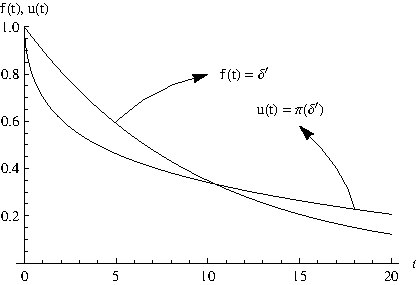
\includegraphics[scale=1.2]{Graph13.pdf}
\captionsetup{width=240pt}
\caption{The exponential discount function f(t) and the function u(t) obtained by applying the mapping from equation \ref{eq:myWeight} to f(t) with $\delta=0.9$ and $\gamma=0.6$. It seems u(t) follows the economist's definition of 'hyperbolic'.}
\label{fig:Graph13.pdf}
\end{center}
\end{figure}

As can clearly be seen, the function which arises from applying probability weights to the exponentially decaying discount function has the feature that it makes a large drop from the present into the near future, while only smaller drops between periods further into the future. The second of the three key points that this paper wishes to propose is that there may be an intimate connection between probability weighting and the particular shape of the discount function. Potential mechanisms behind this connection will be analysed in order to give credit to our idea. Besides making argumentative sense, the benefit of this idea is that the underlying discount function is, in fact, exponential\footnote{One account by Rogers suggest the underlying exponential function discounts future rewards by about 2 percent per year \cite{Rogers1994}. This is based on the fact that future rewards often benefit one's offspring, who are genetically only partially related to you.}. This follows from the constant hazard rate; the chance of not being alive by the time the future reward is realised. As such, when a certain period of time has passed, and you are still alive, you can rescale the objective, discount function to unity, obtain the same exponential function as before and then apply the mapping of probability weights which results in a hyperbolic function. We can say that as time passes, we slide down the exponential function, but look at it through a lens. This lens distorts the image of the smooth exponential function and turns it hyperbolic. Crossing discount functions, dynamic inconsistencies and preference reversals arise naturally.\\
\\
With this striking similarity between hyperbolic discounting and probability weighting, one immediately wonders whether this is a coincidence or whether a deeper force is at play. Part of the purpose of this paper is to investigate this idea. Assuming for a moment that there really is a connection between the two effects, and assuming, as argued above, that evolution is, in fact, responsible for shaping our preferences, there are only three possibilities capable of explaining the observed similarity.
 
\begin{figure}[h]
\begin{center}
\subfloat[There is one single ultimate cause (UC) for both probability weighting (PW) and hyperbolic discounting (HD).]{\label{fig:Graph9.pdf}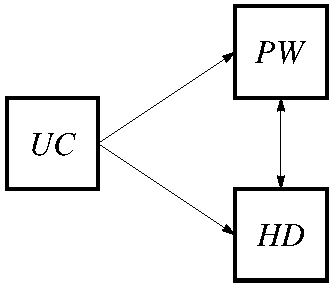
\includegraphics[scale=.5]{Graph9.pdf}}
\hfill
\subfloat[There are multiple ultimate causes for probability weighting and there is only some overlap with the ultimate causes for hyperbolic discounting.]{\label{fig:Graph10.pdf}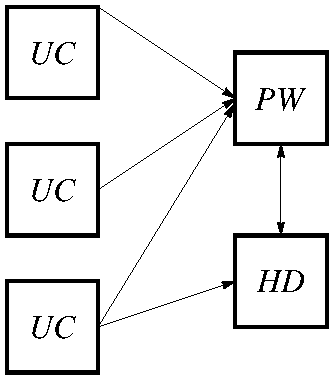
\includegraphics[scale=.5]{Graph10.pdf}}
\hfill
\subfloat[The are two distinct ultimate causes, but both of these share some features, which by a slight abuse of notation we call proximate causes (PC), which are responsible for the similarity between the two effects.]{\label{fig:Graph11.pdf}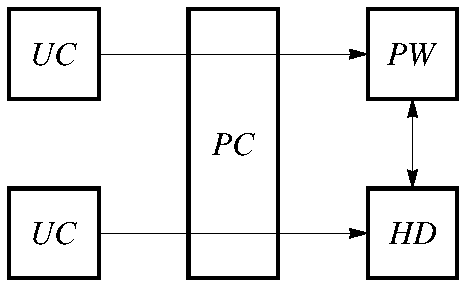
\includegraphics[scale=.5]{Graph11.pdf}}
\captionsetup{width=320pt}
\caption{Graphical representation of the three possibilities concerning the similarity between probability weighting and hyperbolic discounting.}
\label{fig:Graph9.pdf and Graph10.pdf and Graph11.pdf}
\end{center}
\end{figure}

The first of these possibilities is that there is one single ultimate cause for why humans, and some animals, weight probabilities and for why they discount the future in a hyperbolic manner. The second possibility is that there are several ultimate causes for probability weighting, i.e. there are several reasons why it may be advantageous to weight probabilities in an evolutionary setting. It is, then, possible that only one of these causes is also responsible for the type of weighting which is applied to the exponentially decaying discount function, resulting in hyperbolic discounting. Finally, it is possible that there are two distinct ultimate causes for probability weighing and hyperbolic discounting. If this is the case, the similarities between the two effects may only be due to similarities in the features of the two ultimate causes, i.e. there may be a more proximate cause which is identical in both cases, but does not stem from the same underlying mechanism. The last of the three key points this paper wants to address is a model which tries to explain hyperbolic discounting by assuming there truly is an intimate connection between probability weighting and the hyperbolic shape of the discount function.


\section{Evolutionary Psychology}
\label{sec:Evolutionary Psychology}
\subsection{Fitness Equals Utility}
\label{sec:Fitness Equals Utility}

In the same way as that physics is needed to understand chemistry and chemistry is needed to understand biology, psychology is needed to understand economics. It is the purpose of evolutionary psychology to complete this list by finding the missing link between biology and psychology. Once this is established, much of economics may be explained from first principle, with less need for premises and assumptions.\\
\\
The most fundamental insight, which lays at the heart of evolutionary psychology, is that happiness or utility is our body's way of controlling our actions. In fact, it is the long reach of the gene, which determines our behaviour in a way that is optimal for the genes. For example, people enjoy sex; they derive utility from it. This mechanism ensures we repeat the behaviour many times, increasing our genes' chance of survival. In this way, the behaviour which gives us utility also gives us a higher biological fitness. But utility is derived from many other things as well, such as eating or consuming goods and resources. If utility does, in fact, equal biological fitness, and we seek to maximise our utility, we ultimately end up maximising our fitness. It may seem surprising that evolution is capable of calculating which actions enhance our fitness, but explaining complexity from simplicity is the prime achievement of the theory of evolution by natural selection. One example to show how good evolution can be at producing optimal behaviour comes from an experiment with woodpeckers. In this experiment, woodpeckers had to determine how many holes in a tree to try for food before accepting that that tree did not contain any food and move on to the next one. The average number of holes tried by the woodpeckers was remarkably close to the correct number calculated with advanced mathematics and statistics \cite{Wilkinson2008}. This shows that evolution is capable of solving difficult optimisation problems in its attempt to increase our chances for survival.


\subsection{Fitness Does not Equal Utility}
\label{sec:Fitness Does not Equal Utility}

All is well with maximising utility when animals are in simple situations where no strategic interactions need to be taken into account. We can say that in these cases, the animal is playing a game on its own in which maximising utility equates to maximising fitness. Things change, however, when there are multiple players in the game and interdependencies and externalities arise. In those cases, it may be advantageous to back away from the most rational decision, from the strategy which directly maximises utility \cite{Frank1988}. This is because there are some games in which choosing an irrational, sub-optimal strategy may induce a behaviour from the other players which eventually leads to a higher fitness for yourself. We have already encountered an example of such a situation. In the case of loss-aversion, Huck et al. had posited that in a simple Nash-bargaining game, players may obtain a higher pay-off if they value their property higher than would seem rational \cite{Huck2005}. The reason for this was that such loss-aversion leads to toughness in bargaining. This toughness forces the opponent to accept a lower pay-off for himself and, therefore, leads to a higher fitness for the biased player. In such cases with strategic interaction, therefore, maximising a utility function which does not exactly equate to the fitness function, may well end up maximising fitness.


\section{Probability Weighting}
\label{sec:Probability Weighting}
\subsection{Replication of the Model}
\label{sec:Replication of the Model}

We have talked about evolutionary psychology, and its aim to fundamentally understand economic behaviour, in very general terms. Now it is time to investigate a specific model which tries to explain the probability weighting of Prospect Theory from an evolutionary perspective. The following model is based on Rieger's paper 'Evolutionary Stability of Prospect Theory Preferences' which itself drew heavily from Goeree et al. \cite{Rieger2009, Goeree2003}. We combine the model with works by Guth and Von Widekind and some original ideas \cite{Guth1992, Guth1995, Widekind2008}.\\
\\
We will consider a 2 by 2 game matrix which resembles the matching pennies game. Arguments for why these particular pay-offs are reasonable and natural will be presented below, in Section~\ref{sec:What Games are played in Nature}. However, we can already build on the intuition behind the general dynamic of such a matching pennies game. Goeree et al. gives the example of a football goalie who would prefer to dive in the same direction as the ball is shot in, while the opponent prefers to shoot in a different part of the goal than where the goalie dives to. In nature, this type of situation may also have occurred regularly.

\begin{table}[h]
\begin{center}
\[
\begin{array}{r|rr}
  & \text{B1} & \text{B2} \\
\hline
 \text{A1} & 
\begin{array}{ll}
   & 2 \\
 4 &  
\end{array}
 & 
\begin{array}{ll}
   & 3 \\
 -2 &  
\end{array}
 \\
 \text{A2} & 
\begin{array}{ll}
   & 2 \\
 3 &  
\end{array}
 & 
\begin{array}{ll}
   & 0 \\
 0 &  
\end{array}

\end{array}
\]
\end{center}
\caption{Pay-off matrix of the generalised matching pennies game.}
\label{tab:PayoffMatrixPWRep}
\end{table}

In our model, there are two levels, following what is known as the indirect evolutionary approach. The lowest level contains the actually pay-offs to the players in terms of biological fitness. The pay-offs are some reward such as resources or the opportunity to mate and enhance the survival of the player. The level above contains the preferences over the reward. As was explained, in settings of strategic interaction, evolution may favour agents whose utility function does not perfectly trace its fitness function. We allow various types of players in our model to have all possible preferences over the rewards and let natural selection decide which type has the most advantageous preference profile. It is assumed that, given their utility function, the various types act 'rational' in the sense that they try to maximise their utility. This need not coincide with the direct maximisation of fitness. However, it is the fitness which in the end determines which type will become dominant in the population as the mechanism of evolution is such that those with the highest fitness produce the largest number of offspring and will therefore become relatively more numerous.\\
\\
To make this model more precise for our analysis, take the weighting function in Equation~\ref{eq:myWeight}. The distinction between the types of people in our model is determined by the weighting variable $\gamma$. In the setting which we will describe below, the type with the optimal level of probability weighting will emerge dominant in the population. To allow for a richer variety of weighting, let us go beyond Rieger's model and extend this equation to the following:

\begin{equation}
\label{eq:myWeight2}
\pi(p, \gamma, \lambda, \mu)=\frac{p^{\gamma}}{(p^{\lambda}+(1-p)^{\lambda})^{1/\mu}}
\end{equation}

In this case, the distinction between the types of people is determined by the weighting variable $\gamma$, as well as the variables $\lambda$ and $\mu$. The reason why the two exponents on the probabilities $p$ and $1-p$ are the same is the symmetry in the function\footnote{By including even more variables in our equation, we could model higher order deviations from the linear, objective probability function. However, this level of complexity is unnecessary, especially seeing the fact that we already know what behaviour should come out of the model. Empirical data suggests the deviation is of order two, with overweighting of low probabilities and underweighting of high ones.}. The four possible behaviours in terms of weighting probabilities are shown in Figure~\ref{fig:Graph2.pdf}. What we then hope to find through our model is that only one of these possible behaviours survives the evolutionary process.

\begin{figure}[h]
\begin{center}
\leavevmode
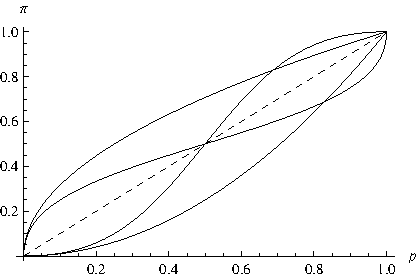
\includegraphics[scale=1]{Graph2.pdf}
\captionsetup{width=290pt}
\caption{The four possible behaviours in terms of weighting probabilities: General overweighting, general underweighting, underweighting low probabilities while overweighting high ones and overweighting low probabilities while underweighting high ones.}
\label{fig:Graph2.pdf}
\end{center}
\end{figure}

The game described above has no pure strategy equilibria. It does have a mixed equilibrium, where both players A and B choose their first strategy with probability $\frac{2}{3}$ and their second with probability $\frac{1}{3}$. This is exactly what we need if we want to consider the effects of weighting on probabilities. According to the strategy chosen by their opponent, the players know they will end up in either one of two outcomes. We assume that the players weight the probabilities with which they believe their opponent chooses his strategies. In this case, the players will not end up in the objective mixed equilibrium, but in a different equilibrium, based on their level of probability weighting. To see precisely how the players do this, look at the following equation which determines the subjective utility a player gets from a particular outcome.

\begin{equation}
\label{eq:myUtility}
\begin{array}{rcl}
u_A(\sigma_A)&=&\sum_{\sigma \in \sum} \sigma_A \pi(\sigma_B) f(\sigma)\\
 &=&4 p_A \pi(p_B) - 2 p_A \pi(1-p_B) + 3 (1-p_A) \pi(p_B)
\end{array}
\end{equation}\\

In this equation, the utility of A is determined by his own mix of strategies $\sigma_A$ as well as the mix of strategies by player B, $\sigma_B$. These latter probabilities are weighted using the weighting function $\pi(p)$. As such, the utility one feels from a particular strategy is not necessarily equal to the fitness one gets from that outcome. Whereas the fitness of an outcome is determined by the rational expected utility theory\footnote{Or should we say, expected fitness theory?}, using objective probabilities, the utility deviates from this following the players beliefs due to probability weighting.\\
\\
Just as there are two levels in terms of fitness and utility, there are also two levels in this model related to the speed at which the game is played and at which evolution selects the optimal preference profile. We assume that the game is played much faster than the speed at which evolution operates \cite{Rieger2009}. That means that, from the point of evolution, the game is always in its equilibrium. This is an adiabatic approximation.\\
\\
There are two ways to justify the idea that the game will always be in its equilibrium position. First, we can say that the players repeat this game several time over, such that they can learn quickly what type their opponent is. As such, they will know what mixed strategy is optimal for them. Particularly, the opponent will know how to adjust his mixing of strategies so as to compensate for the 'irrational' behaviour by the other player. Alternatively, we can follow Von Widekind and Dekel et al. by assuming that the type of the players is known to the other player, i.e. one can observe the type and play the optimal strategy immediately \cite{Widekind2008, Dekel2007}. For the first of these two alternatives, the dynamics of the strategy space can be analysed\footnote{The following graphs, as well as all the calculations done in this paper, were produced using a \textit{Mathematica} notebook.}. The replicator equation was originally conceived to describe the dynamics of populations under natural selection, however, it was soon realised that the same equation may also describe a learning process.
 
\begin{figure}[h]
\begin{center}
\subfloat[$\gamma=1$]{\label{fig:Graph3.pdf}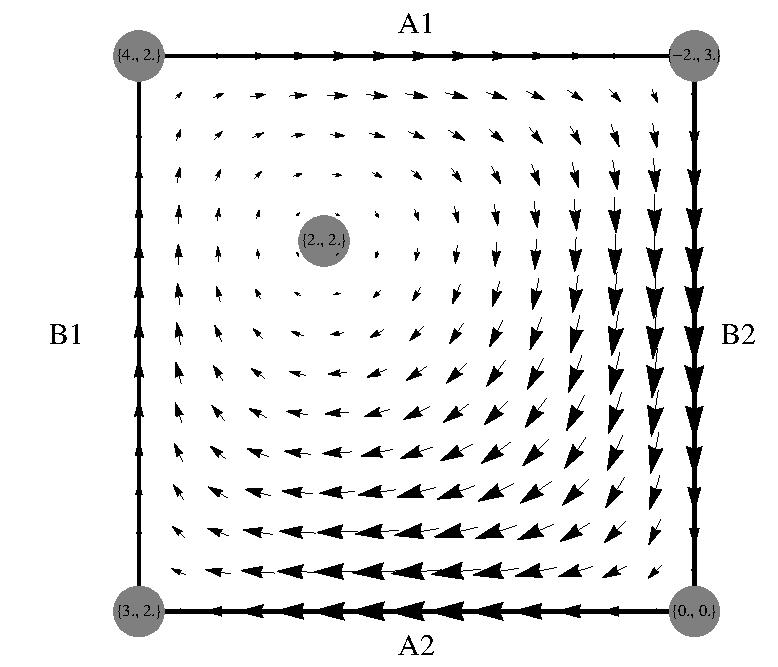
\includegraphics[scale=.58]{Graph3.pdf}}
\hfill
\subfloat[$\gamma=.5$]{\label{fig:Graph4.pdf}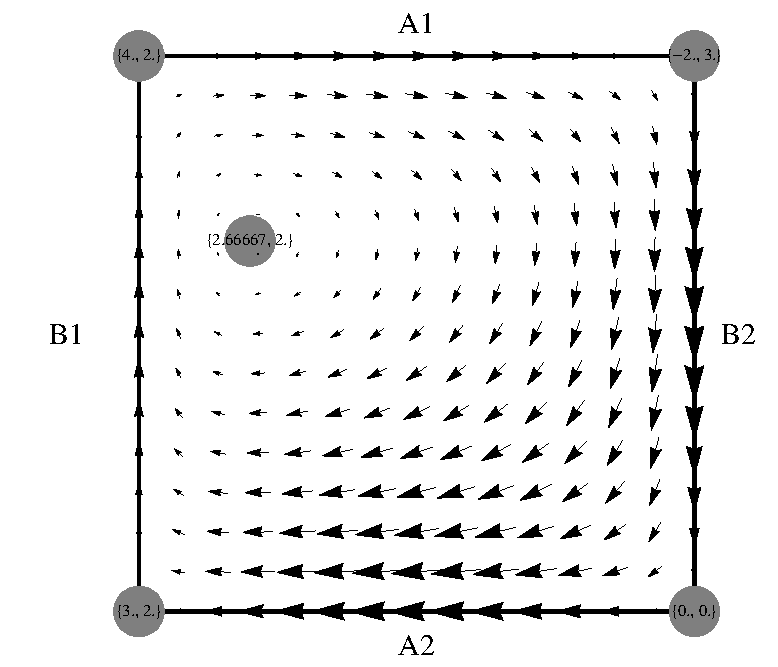
\includegraphics[scale=.58]{Graph4.pdf}}
\captionsetup{width=400pt}
\caption{Strategy spaces with replicator dynamics as a learning process in the generalised matching pennies game.}
\label{fig:Graph3.pdf and Graph4.pdf}
\end{center}
\end{figure}

In Figure~\ref{fig:Graph3.pdf} above, we see the strategy space of the two players and the typical matching pennies behaviour around the mixed equilibrium. In this objective equilibrium, both players obtain a fitness of $2$. If player A, however, weights the probabilities with which he expects player B to choose between his strategies, the position of the mixed equilibrium changes. Goeree et al. applied this idea to experimental data and found that it fit the data well \cite{Goeree2003}. In Figure~\ref{fig:Graph4.pdf} we see the dynamics change slightly when player A weights\footnote{As we shall see later on, the values of $\lambda$ and $\mu$ are irrelevant for this result.} with $\gamma=0.5$. The mixed equilibrium has now shifted, specifically towards to outer sides of the strategy space. The shift in the equilibrium is advantageous\footnote{In the more general model developed by Von Widekind, the author also finds that under the indirect evolutionary approach, the population becomes dominated by a type which always plays the strategy with the highest fitness level, and therefore the most efficient outcome, if the players can observe the opponent's type \cite{Widekind2008}.} for player A, who now obtains a fitness of $2.67$. In fact, for a very general pay-off matrix, the subjective mixed equilibrium is positioned at:

\begin{equation}
\label{eq:myProspectSolveA}
\alpha \to \frac{(\text{b3}-\text{b4})^{\frac{1}{\gamma }}}{(\text{b1}-\text{b2})^{\frac{1}{\gamma }}+(\text{b3}-\text{b4})^{\frac{1}{\gamma }}}
\end{equation}

\begin{equation}
\label{eq:myProspectSolveB}
\beta \to \frac{(\text{a2}-\text{a4})^{\frac{1}{\kappa }}}{(\text{a1}-\text{a3})^{\frac{1}{\kappa }}+(\text{a2}-\text{a4})^{\frac{1}{\kappa }}}
\end{equation}\\

Here, we call the level of probability weighting by player B $\kappa$ and not $\gamma$ to avoid confusion between the two different players. What is striking about this result, however, is that the variables $\lambda$ and $\mu$ have literally dropped out of the equation\footnote{The reason that $\lambda$ and $\mu$ are irrelevant in the determination of the position of the mixed equilibrium is that the denominator is perfectly symmetric in $p$ and $1-p$. What matters in the model is only the relative value of $\pi(p)$ and $\pi(1-p)$. As such, the entire denominator drops out.}. This means we are able to see the effect of changing $\gamma$ but still have no idea about optimal values for $\lambda$ and $\mu$. We see that a lower $\gamma$ leads to a higher fitness. As such, there will be an evolutionary pressure towards a lower $\gamma$. We can cross out two of the general types of behaviour found in Figure~\ref{fig:Graph2.pdf}, namely, those for which $\gamma>1$. What remains possible in the model is a general overweighting of all probabilities or an overweighting of only low probabilities and underweighting of the high ones, depending on the precise values of $\lambda$ and $\mu$. The properties of this model which account for the increase in fitness will be analysed later, in the Section~\ref{sec:Appropriate Properties}.

%Let us first consider a slight variation of this game to see whether we can extend the class of generalised matching pennies games to a wider variety.

%\subsection{Variation}
%\label{sec:Variation}

%For a 2 by 2 game, most pay-off matrices lead to a strategy space with only pure equilibria. There are two classes of games which have a mixed equilibrium. The matching pennies class above is one example, the class resembling the hawk-dove game is the other. In this class, however, there are two pure strategy equilibria as well, in which the game can end up. In the typical hawk-dove example, it is assumed that the two players are correlated in the sense that they are identical. This means that there is a symmetry in the game which does not allow the final equilibrium to be off the diagonal. To see this more clearly, consider ... . If players A and B entered this type of game repeatedly before learning what type the opponent was, there is a possibility that they would end up in one of the pure equilibria. As this is not what we are looking for, in this class we need to impose an additional restriction. ... . Figure~\ref{fig:Graph5.pdf and Graph6.pdf} below shows the strategy space of this class of games.
 
%\begin{figure}[h]
%\begin{center}
%\subfloat[$\gamma=1$]{\label{fig:Graph5.pdf}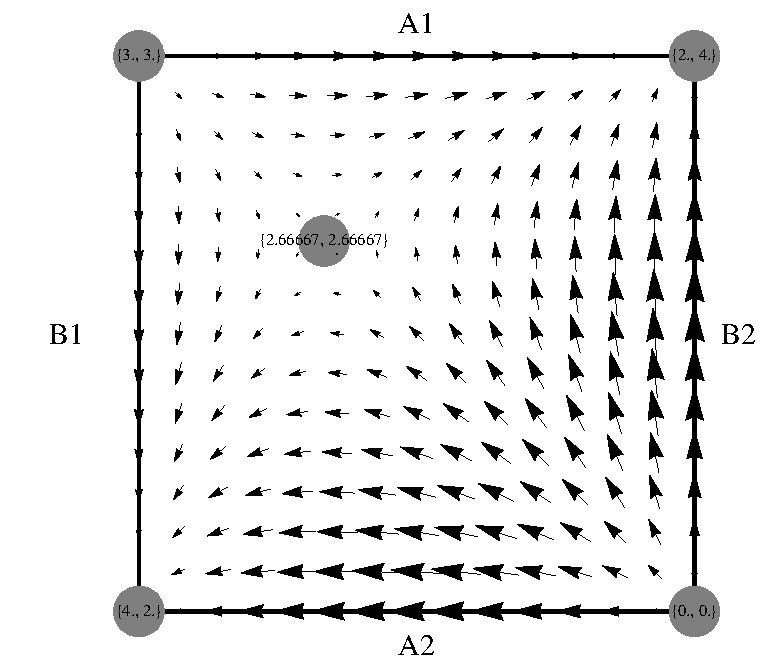
\includegraphics[scale=.5]{Graph5.pdf}}
%\hfill
%\subfloat[$\gamma=.5$]{\label{fig:Graph6.pdf}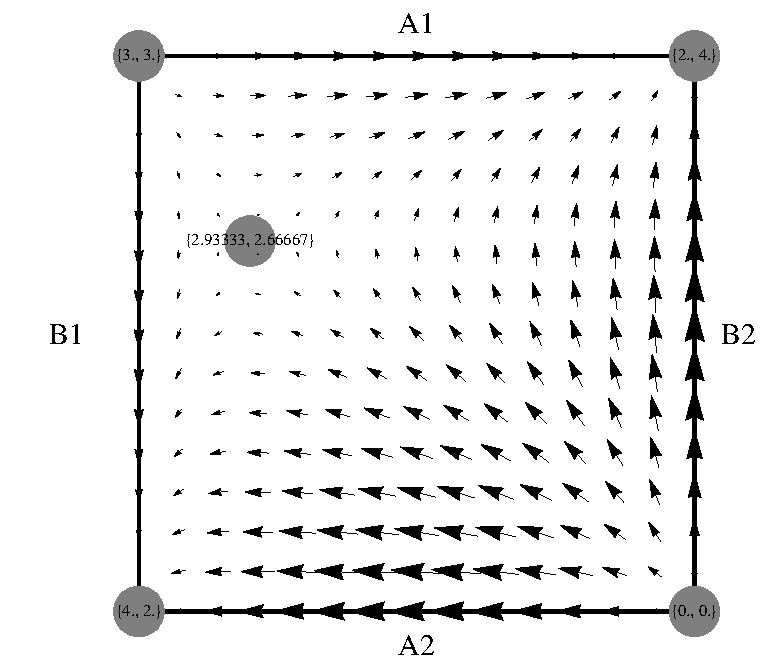
\includegraphics[scale=.5]{Graph6.pdf}}
%\captionsetup{width=330pt}
%\caption{Strategy spaces with replicator dynamics as a learning process in the hawk-dove game.}
%\label{fig:Graph5.pdf and Graph6.pdf}
%\end{center}
%\end{figure}

%As can be seen, the weighting of probabilities can once again lead to a higher fitness.


\subsection{Extension of the Model}
\label{sec:Extension of the Model}

The original paper by Rieger shows that a population of probability weighters is evolutionarily stable, i.e. stable against the infiltration of a mutant who weights less \cite{Rieger2009}. We have shown the equivalent by demonstrating that a player with a higher level of probability weighting will obtain a higher fitness. Types which receive a higher fitness will grow in number in the population. By showing that the fitness will always increase for a higher degree of weighting, we have proven that no mutant with a lower level of weighting can infiltrate in the population and that the high weighting type will dominate in the long-run. Unlike Rieger, however, our argument is not based on the notion of group selection for which probability weighting is beneficial to the group as a whole\footnote{Rieger also applies his probability weights to the 'War of Attrition' game to show that is will lead to lower waiting times for both players, which is beneficial in terms of getting a higher pay-off \cite{Rieger2009}. However, this argument, as well, is based on group selection and does not hold. A mutant with a lower level of probability weighting would be able to wait a little bit longer than the other players and thereby obtain all the benefits. Although a population of such low weighting players would receive smaller pay-offs than an entire population of high weighter, it is the only type of population which is stable under true evolution at the gene-level.}. We have shown that even the selfish gene would favour a higher level of weighting, because the shift in the position of the mixed equilibrium causes an increase in the fitness of the player. As such, one would expect the process of increasing probability weights to continue until $\gamma=0$. Rieger argues, however, that such a jump away from the more rational, true probabilities would not be beneficial to an animal in the end as the class of games described above is not the only game he will encounter in Nature \cite{Rieger2009}. As we mentioned, a utility function which does not perfectly trace the fitness function may be beneficial under strategic interactions, but will certainly not be beneficial in all situations, for example, where there is no strategic interaction. A realistic picture of evolution is a setting in which an animal plays several types of games, with and without strategic interactions, and applies a level of probability weighting which is optimal for such a combination of games. Figure~\ref{fig:Graph8.pdf} below sketches a simple version of this idea, in which a player either ends up playing the matching pennies game or ends up playing a simple game where applying correct probabilities is advantageous. An example of the latter game is a situation in which an animal has the choice between a nearby tree with average food and a further-away tree which may or may not have very good food. The application of correct probability estimates is very important here, as it will have an effect on the quality of the resources you can consume and, therefore, on the chances of survival.

\begin{figure}[h]
\begin{center}
\leavevmode
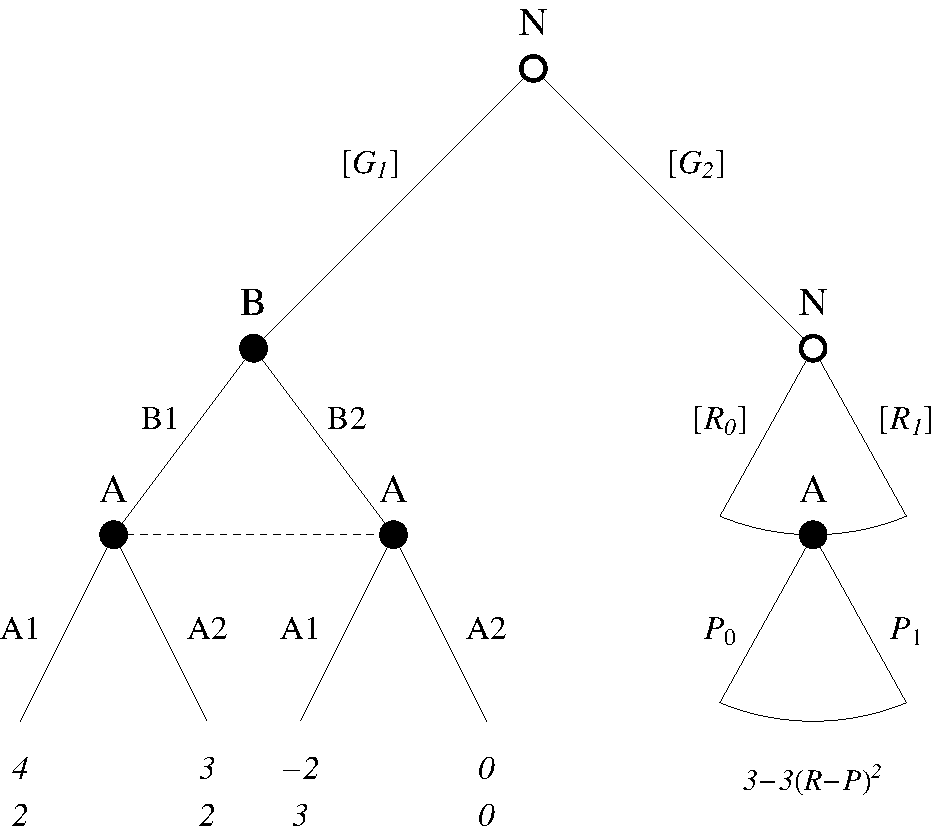
\includegraphics[scale=.52]{Graph8.pdf}
\captionsetup{width=360pt}
\caption{Animals encounter various kinds of games. With density $[G_1]$, they will play the matching pennies sub-game, with density $[G_2]$, they play a simple, one-player game, in which it is important they judge the probability $R$ accurately.}
\label{fig:Graph8.pdf}
\end{center}
\end{figure}

The extensive form above has particular pay-offs and a particular density of which game is played, but what is most important is the general notion that probability weighting may be advantageous in some situation while disadvantageous in others. As such, there is some level of probability weighting, which will be between $\gamma=1$ and $\gamma=0$, which is optimal for the environment as a whole. If we combine the two sub-games with $50$-$50$ probability, the following fitness will be obtained for various levels of $\gamma$.

\begin{figure}[h]
\begin{center}
\leavevmode
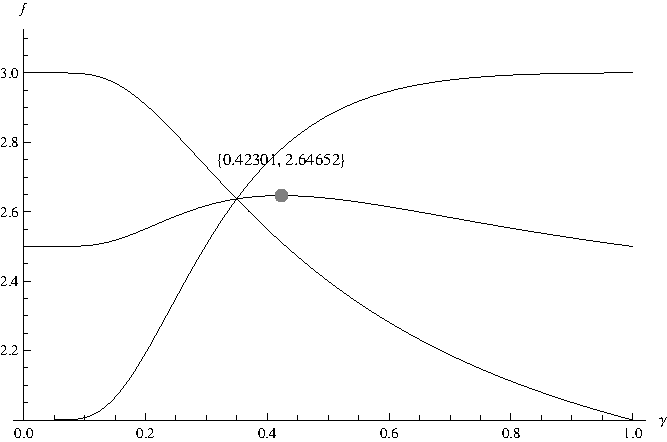
\includegraphics[scale=.68]{Graph7.pdf}
\captionsetup{width=360pt}
\caption{The two sub-games in our extension of Rieger's model, for which we have used weighting as in Equation~\ref{eq:myWeight}, give a different response in terms of fitness to decreases in $\gamma$. Whereas in the matching pennies sub-game the fitness increases with lower levels of probability weighting, the fitness decreases for our simple, one-player game. A combination of the two, in this case with equal densities, shows what the total fitness will be and for what level of $\gamma$ this reaches its maximum.}
\label{fig:Graph7.pdf}
\end{center}
\end{figure}

As can be seen, the pay-off of the matching pennies game increases when $\gamma$ decreases, while for the other game, the benefit becomes lower. The total fitness obtained is highest for a $\gamma$ somewhere in between $0$ and $1$. This gives us a notion of what kind of probability weighting is evolutionarily stable. We see that a population which does not weight at all may be infiltrated by a probability weighter with a lower $\gamma$ because the person with the lower $\gamma$ obtains a slightly higher fitness. Likewise, a population for which $\gamma=0$ is also not evolutionarily stable, as a lower degree of probability weighting leads to a higher fitness. The evolutionarily stable state of this model is found for values of $\gamma$ somewhere in between these two extremes.\\
\\
What is more important, however, is that this approach gives us a clear answer for the values of $\lambda$ and $\mu$. As these variable did not enter the equation of the position of the mixed equilibrium in our matching pennies game, they were, up until now, still undetermined. As such, we were not yet able to decide which of the four possible methods of weighting, described in Figure~\ref{fig:Graph2.pdf}, would survive the evolutionary process. Using our extension, however, we obtain the optimal values of $\gamma=0.13$, $\lambda=0.31$ and $\mu=0.80$. We can say that the only evolutionarily stable state of our model is given by these three values. The most important notion that this gives is that, like $\gamma$, $\lambda$ and $\mu$ lie somewhere between $0$ and $1$. From the original four possibilities found within Equation~\ref{eq:myWeight2}, we had narrowed it down to two, for which $0<\gamma<1$ while $\lambda$ and $\mu$ were undetermined, by applying Rieger's model. Now we are left with just one possibility following our extension. Only those types of people who overweight low probabilities and underweight high probabilities will dominate in the long-run.


\section{Hyperbolic Discounting}
\label{sec:Hyperbolic Discounting}
\subsection{Appropriate Properties}
\label{sec:Appropriate Properties}

We have seen some similarity between probability weighing and hyperbolic discounting by showing that someone who applies weights to the probability of the realisation of a reward in the future will end up with a hyperbolic discount function. We have also shown one particular model which can explain the existence of probability weighting from an evolutionary perspective. If it is true that the ultimate cause of this probability weighting is also responsible for the hyperbolic discount function, we should try to analyse what properties of the previous model exactly result in the increase in fitness for probability weighters.\\
\\
The most important property which results in an increased fitness is one very much related to a credible threat. Imagine the two players start in the mixed equilibrium of the game. If player A is a probability weighter, he will misjudge the action of his opponent B and believe it to be appropriate to move downwards on his strategy space. He will feel that it is optimal to choose his strategy A2 more often. In reality, however, this is irrational as it would result in a lower fitness. To be more precise, the strategy A2 is not the only best-reply to the strategy of player B. However, as there is interdependency between the players, this move by A will cause B to also shift his strategy. He will respond to the threat by A by moving more closely to his first strategy, B1. This shifts the mixed equilibrium towards the outer side of the strategy space and results in a higher pay-off to player A. Take the example of the goalie. By choosing one corner more often, he induces a reaction from his opponent to shoot in the other corner more often. If the pay-offs are such that this response actually benefits the goalie, his initial 'irrational' behaviour ends up benefitting him.\\
\\
At the position of this new mixed equilibrium, the equilibrium in the higher-level, subjective game, it would be rational for player A to choose his strategy A1 more often. However, for the same reason, player A misjudges his opponent's actions and decides not to move away from his mix of strategies. Irrationally, he decides to continue mixing his strategies A1 and A2 with probabilities $\frac{2}{3}$ and $\frac{1}{3}$. This is ultimately a good thing, because otherwise player B would also need to adjust his strategy, resulting in a return to the original equilibrium in which player A obtained a lower fitness.


\subsection{Inappropriate Properties}
\label{sec:Inappropriate Properties}

There are also properties of the model which are essential for the type of probability weighting we tried to explain earlier, but which will prove inappropriate for explaining hyperbolic discounting. As we shall see in the next section, a direct interpretation of this model as one of future discounting turns out to be impossible, or at the very least, unreasonable, due to these properties.\\
\\
When player A applies probability weighting, he does so on the strategy of his opponent and on both $p$ and $1-p$. He sees that player B will choose between one of two alternatives, B1 or B2. There is a perfect symmetry between these to strategies. The pay-off for players A and B may not be the same, but whatever B chooses, A will receive some pay-off and B will receive some pay-off. If B mixes between his two strategies, player A will obtain the reward associated with strategy B1 discounted by the probability of him choosing that strategy. At the same time, he will obtain the reward associated with strategy B2, discounted by the probability of him choosing B2. As player B moves his strategy from B1 more towards B2, A will receive the reward associated with strategy B2 with an increasingly higher discount factor, until he receives it with certainty when B move all the way to the right. The important thing to take from this is that A will always obtain a reward and that it does not matter which part we call 'B1' and which 'B2'. There is a symmetry in the names, just as there is a symmetry in the probabilities: it does not matter whether we redefine $p \to 1-p$, the model will still be the same and both probabilities will still be weighted, resulting in the same subjective probabilities and the same mixed equilibrium.


\subsection{Direct Interpretation}
\label{sec:Direct Interpretation}

To see what is so important about the symmetry between the names of the strategies, and likewise the symmetry between the probabilities $p$ and $1-p$, let us consider the same game as above, but reinterpreted to include future discounting. As we saw in the introduction, there may be an intimate connection between probability weighting and hyperbolic discounting following the similarity between discounting future rewards due to uncertainty about their realisation and discounting gambles due to the inherent uncertainty within the gamble. If the previous model is capable of explaining probability weighting from an evolutionary perspective, it may also be able to explain hyperbolic discounting if we simply reinterpret the variables of the model and the strategies of the players.\\
\\
Initially, the probabilities $p$ and $1-p$ associated with mixed strategies were viewed as the chance of the realisation of the two pay-offs, determined by the actions of the players. Now, these variables should be viewed as the probabilities of the realisation of a reward after some period of time which is uncertain due to the hazard rate. As such, the axes on the strategy space now no longer represent mixed strategies, but are time variables. Players A and B each choose a time $t_A$ and $t_B$ within this reinterpretation of the game.

\begin{figure}[h]
\begin{center}
\leavevmode
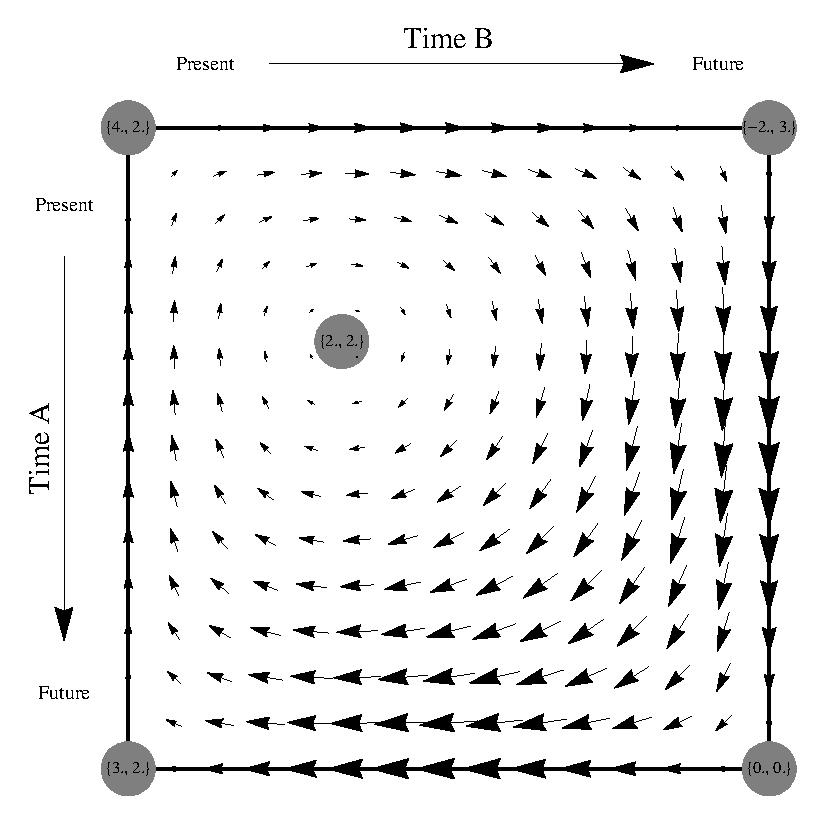
\includegraphics[scale=.57]{Graph14.pdf}
\captionsetup{width=360pt}
\caption{The strategy space of the model by Rieger, but reinterpreted such that the probabilities of a strategy being chosen are now probabilities of still being alive at some time $t$ in the future.}
\label{fig:Graph14.pdf}
\end{center}
\end{figure}

The further into the future the reward will be available, the less likely it is that you will obtain it. As such, the reward is discounted according to the probability of realisation. If player A would obtain a fitness of $4$ at (A1, B1), he would get $4 \times \delta ^{t}$ if player B moves $t$ steps to the right within his strategy space. This is not very different from the original model. If player B moved to the right, away from his strategy B1, the probability of B1 occurring was less and player A had to discount the associated pay-off more. However, to follow the model above accurately, we need to acknowledge that while the chance of still being alive to see the first rewards realised decreases with time, the chance of being dead increases. The original interpretation of this was that when player B moved to the right, the probability of strategy B1 occurring may have decreased, but the probability of B2 occurring would subsequently increase. This means that, when we move to the right on the strategy space, the benefit of the first reward becomes lower, while we would need to consider the benefit of the second reward, the one associated with (A1, B2), to be increasing. In some way, we would need to associate a benefit to being dead which has an increasing present value further into the future, as the probability of being dead is higher there. We see that the symmetry between the two strategies B1 and B2 of player B is no longer valid in this case, because there is no natural symmetry between being dead and alive. Biological advantages can only be included in the fitness while being alive. There is no advantage to being dead and, therefore, we cannot give an interpretation to the pay-off originally associated with strategy B2 in this variation on Rieger's model. Likewise, we could not simply redefine $p \to 1-p$ and expect nothing to change. If $p$ is the probability of still being alive after some period of time and $1-p$ is the probability of being dead, redefining these two terms would give vastly different results. A direct interpretation of the model for probability weighting in terms of future discounting seems impossible due to this property. If it where not impossible, the equivalent result as before would follow in that players benefit from hyperbolic discounting by its effect on the position of the equilibrium.


\subsection{Indirect Interpretation}
\label{sec:Indirect Interpretation}

We have discussed above in what way the similarity between probability weighting and hyperbolic discounting can be explained from an evolutionary perspective. There were three alternatives, of which the first suggested that the ultimate cause for both effects was the same, Figure~\ref{fig:Graph9.pdf}. We can now cross out this possibility. What remains is that there are different ultimate causes for the effects and that only some of them overlap. This is not ruled out, though we can say with certainty that the particular model developed by Rieger to explain probability weighting is not appropriate for explaining hyperbolic discounting. There may be other models which explain not only probability weighting, but also hyperbolic discounting. Further research into whether other models for probability weighting can be reinterpreted as models of future discounting still needs to be done, but with such a striking similarity between the two effects, it is a promising approach. Finally, there was another possibility which explained the similarity between probability weighting and hyperbolic discounting. This was based on the idea that there were two distinct ultimate causes, two distinct models, but that they shared some properties which may lead to the effects. We have already discussed such a property: the credible threat.\\
\\
In the case of loss-aversion, we saw that a certain level of toughness in bargaining may be advantageous as it shifted the equilibrium solution in favour of the tough player. As Huck et al. point out, the individuals behave sincerely and truly follow their preferences; they do not lie nor commit a non-credible-threat, they simply develop an innate sense of loss-aversion 
\cite{Huck2005}. In the case of probability weighting, we saw that by misjudging the probabilities with which the opponent chose his strategies, the player was led to engage in a threat. This threat was credible because the player really did feel his subjective probabilities were correct, he was not merely pretending to obtain a better outcome. Can we come up with a situation in which hyperbolic discount may lead a player to put out a threat towards his opponent? A threat which in first instance may seem irrational because it would lead to a lower pay-off, but ultimately proves beneficial because of the adjustments made by the opponent.\\
\\
Consider a situation similar to the ultimatum game. Two players own a particular good which gives them a benefit equal to $\frac{1}{4}$ on every time period. The present value of this good can be evaluated by integrating over time, discounted for the probability of dying in the future. However, it turns out that when both these goods are combined, their total benefit is equal to $1$. One example could be that one player owns a long stick while the other owns a sharp blade. Used together, these goods for a very useful spear. As such, it would be beneficial to both players if they could decide on a sharing plan. Player A would obtain the two goods first, for a certain amount of time $t$, before giving them both to player B. Player B would enjoy the benefit of the goods for the remainder of the time.

\begin{figure}[h]
\begin{center}
\leavevmode
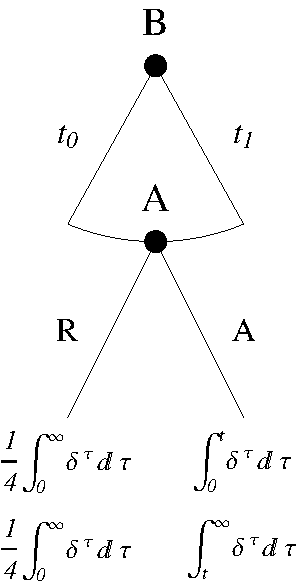
\includegraphics[scale=.68]{Graph12.pdf}
\captionsetup{width=380pt}
\caption{Both players own a good which benefits them in every period, conditional on them still being alive. If they share the goods by letting A have them both for a length of time $t$ and B for the remainder of the time, they may both benefit more. Player B makes an offer of this length of time $t$ which A can either accept of reject.}
\label{fig:Graph12.pdf}
\end{center}
\end{figure}

It is up to player B to decide on the time period $t$ for which player A is allowed to hold the two goods. Player A merely has to accept the offer, or reject it. If we assume, for simplicity, that $\delta=0.9$, the benefit to both players when A rejects the offer is $9.49$. As such, if under the sharing plan A can get a higher benefit, he should accept the offer. When one follows the calculations, it seems that A should accept the offer whenever $t>2.73$. Similarly, B would benefit from the exchange whenever he obtains the two goods before $t=13.16$. To maximise his profit in this ultimatum game, B should offer $t=2.73$, which A should accept. However, if A is not perfectly rational, if A discounts the future in a hyperbolic fashion, the result may be different. Let us assume that A follows a hyperbolic function such as in Figure~\ref{fig:Graph13.pdf} with a $\gamma=0.6$. A is now of the opinion that he will not benefit from an exchange in which he is only allowed to use the two good for a time period of $t=2.73$, so he rejects that offer. A is making a threat towards player B, one which is credible because A truly believes he has acted rationally. If we redo the calculation, it now seems that A would only accept offers from B where $t>3.66$. As this length of time is still below the maximal level B would accept, B is very willing to make this offer. As such, the fact that player A has engaged in hyperbolic discounting has led him to receive a higher pay-off and obtain a higher biological fitness. Players such as A, who show hyperbolic discounting, will then increase within the population.\\


\section{Limitations}
\label{sec:Limitations}
\subsection{What Games Are Played in Nature}
\label{sec:What Games Are Played in Nature}

We have now seen that the model by Rieger, with our extension, is very capable of explaining probability weighting. We have seen that there is only one type of weighting, for a particular $\gamma$, $\lambda$ and $\mu$, which gives the optimal fitness level. However, all of this is based on the idea that the type of game presented by Rieger was common in the history of our ancestors.\\
\\
The idea of the matching pennies game is simple. In general, it may be true that one player benefits from a match, while the other player benefits from a mismatch. We presented the example by Goeree et al. of the football goalie above, who would prefer to dive in the same direction as the ball is shot in, while the opponent would prefer to shoot in a different part of the goal than where the goalie dives to. Rieger explains his generalised matching pennies games as one of social control. In this game, player B needs to cooperate with player A, but also has the option of defecting. Player A has the task to check on B, but this checking comes at a cost. Plugging in some values for these four strategies according to the description, one ends up with the pay-off matrix in Table~\ref{tab:PayoffMatrixPWRep}. Does this story sound reasonable? Would such situations really occur in Nature?\\
\\
We had already discussed that humans and other animals encounter various types of games, some with strategic interaction and some without. We created a model in which Nature chooses which game we play with a certain probability as in Figure~\ref{fig:Graph8.pdf}. To be more realistic, we would need to extend this model by including a wide variety of sub-games; not only 2 by 2 games, but even some with many more strategies and many more players. The appropriate density on each of the sub-games would then allow us to determine the optimal level of probability weighting. This is, of course, a daunting task and our simple model may be very close to the reality of life in the prehistory. At the very least, it illustrates the principle. However, it remains a strong simplification which suggests we should take the final results of our analysis with a grain of salt.

%\subsection{Different Weights and Discount Factors}
%\label{sec:Different Weights and Discount Factors}

%Another limitation of our model is that it only predicts one level of probability weighting. The same degree of weighting is then applied to all situations and the players are not able to switch off this weighting in situations, or sub-games, where it may not be beneficial. Similarly, it is assumed that the discount factor is equal in all situations and that the degree to which the discount function is hyperbolic is also determined by a fixed $\gamma$.\\
%\\
%Experiments have shown that in different situations, people discount the future in a different manner. For example ... \cite{Wilkinson2008}. These effects cannot be explained by our model. In fact, were it allowed to have different levels of weighting or discounting, the analysis in Section~\ref{sec:Extension} would no longer hold. Here, we discussed that animals would not continue increasing their level of probability weighting until $\gamma=0$ because there were other games in which it was necessary for the probabilities to be estimated accurately. If animals where capable of making a distinction between these two situations, they would be able to choose the appropriate level of weighting in both cases separately. Experiments which show that people are indeed capable of having different levels of weighting and different levels of discounting, therefore, present a major problem for our model.


\subsection{Multiple Self}
\label{sec:Multiple Self}

There have also been experiments conducted on future discounting in neuroscience \cite{McClure2004}. These suggest that there are two separate systems in the brain which are responsible for short-term and long-term discounting. The notion that there are multiple selves which deal with various calculations of the present value of a future reward does not agree with our idea that the discount function is hyperbolic due to probability weighting. What the ultimate cause is of this division between the short-term and the long-term system is yet to be discovered and whether hyperbolic discounting follows from this division may be too soon to tell, but this discovery certainly casts doubts on the conclusions of our model.


\subsection{Learning Quick Enough or Observing}
\label{sec:Learning Quick Enough or Observing}

Another aspect of our model which may be regarded as a weakness is its assumption that the two players in the matching pennies game will know what type their opponent is. We have suggested two mechanisms for this; namely that the two players repeat the game several times such that they learn how their opponent plays and what their own optimal strategy is, or that the two players simply immediately observe the type of their opponent. The first of these two mechanisms has the limitation that it is only applicable to a subset of games played in Nature which are indeed repeated several times over. This reduces the likeliness that the game we have been considering is truly a reasonable game to hold as representative of situations in our evolutionary past. The second of these two mechanisms has the limitation that it requires the two players to be able to observe and identify various types within the population. This is in line with some previous work \cite{Guth1992, Guth1995}. But would humans and animals really be capable of doing this? This is another caveat in our model.


\subsection{Prospect Theory is not Cumulative Prospect Theory}
\label{sec:Multiple Self}

Since the development of Prospect Theory, many advances have been made. Most notably, the idea of probability weighting has shifted from a direct mapping of objective probabilities to subjective probabilities to an indirect mapping through the cumulative distribution function \cite{Tversky1992}. This new approach changes the calculations of our analysis somewhat. Although we have not delved into this matter here, Rieger did apply Cumulative Prospect Theory to his research and found that the discrepancy between the two approaches was only minor \cite{Rieger2009}. However, whether this discrepancy is also minor when we apply the new approach to future discounting remains to be seen in future work.


\subsection{Inflection Point}
\label{sec:Inflection Point}

One last limitation of our extension of the model by Rieger is that it does not explain the position of the inflection point of the subjective weighting function. Various experiments have shown that the point at which the weighting function $\pi(p, \gamma)$ crosses the true probability line is well below $0.5$ and that the area of underweighting high probabilities is much wider than the area of overweighting low probabilities. In our model, the only behaviour that comes out includes an inflection point which is very close\footnote{In fact, for the values of $\lambda$ and $\mu$ we obtained, the inflection point is located at $p=0.51$.} to $\pi(p, \gamma)=p=0.5$. Why it is evolutionarily advantageous to have a weighting function with an inflection point at a lower $p$ remains to be investigated by further research.\\


\section{Conclusion}
\label{sec:Conclusion}
\subsection{Achievements of Evolutionary Psychology}
\label{sec:Achievements of Evolutionary Psychology}

In this paper, we set out to give an evolutionary explanation for both probability weighting and hyperbolic discounting. We have presented a model, mostly based on previous work by Rieger, which shows that people who weight probabilities in the manner suggested by Prospect Theory will achieve a greater biological fitness than people who weight less. As such, there is an evolutionary pressure towards greater levels of weighting. Through our extension, however, we show that at some moment, there will also be a counter-pressure which results in an evolutionarily stable equilibrium position in which a particular level of weighting is applied.\\
\\
Initially, we had shown that there was a striking similarity between probability weighting and hyperbolic discounting. This similarity both made intuitive sense and had the additional feature that it was capable of explaining the strange behaviour of dynamic inconsistent preference reversals. Following our model on probability weighting, we made a suggestion of how to reinterpret this model to become one of future discounting in which hyperbolic discounting became evolutionarily advantageous. However, particular properties of the model by Rieger did not allow for a direct interpretation and we were forced to create a new model which merely presented one aspect of hyperbolic discounting, namely its relation to a credible threat, which could cause it to indeed be evolutionarily advantageous.\\
\\
The most important points that this paper hopes to contribute come in threefold. Firstly, the similarity between hyperbolic discounting and probability weighting and the benefits that this idea presents are key. Secondly, in cases where animals play games both with and without strategic interaction, it can be advantageous to weight probabilities in a particular manner, namely that for which the three variables $\gamma$, $\lambda$ and $\mu$ are between $0$ and $1$. Finally, a direct interpretation linking a model of probability weighting with a model for hyperbolic discounting may be possible, but cannot be found in the matching pennies game suggested by Rieger.\\
\\
One of the prediction of our idea that probability weighting and hyperbolic discounting stem from the same ultimate cause is that the two effects should always be observed simultaneously. This means that we can falsify our idea by finding evidence in the biological world of animals who either weight probabilities or discount hyperbolically, but not both. Further research needs to be done to not only check this claim, but also to deal the various limitation of our model.\\
\\
Behavioural economics has spurred great enthusiasm among economists, not only because of its great successes in explaining economic data, but also because its accomplishments entail a grand sensation of truly understanding the essence of behaviour from the more fundamental psychological tendencies inside the human brain. Evolutionary psychology comes with a similar sensation as it uses the grandest, yet simplest theory ever conceived, evolution by means of natural selection, to understand the human brain from the most basic principles. From simplicity to complexity, evolutionary psychology establishes the link from the fields of physics, chemistry, biology and psychology down to the theory of economics and has the power to explain the rich economic behaviour we observe in the world today.

\newpage

\phantomsection
\label{sec:Bibliography}
\addcontentsline{toc}{section}{Bibliography}
\renewcommand{\refname}{Bibliography\\} 
\bibliographystyle{plain}
\bibliography{Bibliography}

\end{document}